\documentclass[12pt,a4paper,twoside,openright]{book}

\usepackage[USenglish,english]{babel}
\usepackage[utf8]{inputenc}

\usepackage{style/isi_style_lt}

\usepackage{amsmath,amsfonts,amssymb,amsthm}
\usepackage{caption}
\usepackage[usenames]{color}
\usepackage{enumerate}
\usepackage{fancyhdr}
\usepackage{fancyvrb}
\usepackage{float}
\usepackage{graphicx}
\usepackage{indentfirst}
\usepackage{listings}
\usepackage{marvosym}
\usepackage{multicol}
\usepackage{sectsty}
\usepackage{subcaption}
\usepackage{tocloft}
\usepackage[table]{xcolor}
\usepackage{url}
\usepackage{float}

\AtBeginDocument{%
	\renewcommand{\contentsname}{Table of contents}
	\renewcommand\tablename{Table}
	\renewcommand\figurename{Figure}
	\renewcommand{\lstlistingname}{List}
	\renewcommand{\refname}{Ref.}
}

\definecolor{dkgreen}{rgb}{0,0.6,0}
\definecolor{gray}{rgb}{0.5,0.5,0.5}
\definecolor{mauve}{rgb}{0.58,0,0.82}

\lstset{
  frame=single,
  captionpos=b,
  language=Java,
  aboveskip=3mm,
  belowskip=3mm,
  showstringspaces=false,
  columns=flexible,
  basicstyle={\small\ttfamily},
  numbers=none,
  numberstyle=\tiny\color{gray},
  keywordstyle=\color{blue},
  commentstyle=\color{dkgreen},
  stringstyle=\color{mauve},
  breaklines=true,
  breakatwhitespace=true,
  tabsize=3
}

\makeatletter
\def\cleardoublepage{
	\clearpage\if@twoside \ifodd\c@page\else
	\hbox{}
	\thispagestyle{empty}
	\newpage
	\if@twocolumn\hbox{}\newpage\fi\fi\fi
}

\makeatother

\setlength{\textwidth}{14cm}
\setlength{\textheight}{21cm}
\setlength{\footskip}{3cm}

\setlength{\hoffset}{0pt}
\setlength{\voffset}{0pt}

\setlength{\oddsidemargin}{1cm}
\setlength{\evensidemargin}{1cm}

\universita{Alma Mater Studiorum -- Università di Bologna}

\campus{Campus di Cesena}
\scuola{}
\corsodilaurea{}

\titolo{Fanta Analytics}

\materia{Sistemi di Supporto alle Descisioni}

\laureando{Gabriele Guerrini, \\ Salvatori Riccardo, \\ Salvatori Stefano}

\annoaccademico{2019 -- 2020}

\makeindex

\begin{document}

\frontmatter 

\maketitle

\tableofcontents

\mainmatter

\pagestyle{fancy} 
\fancyhead[LE,RO]{\thepage}
\fancyfoot{}

\chapter {Data retrival and cleaning}

\section{Data retrival}
Votes for each season since 05/06 are stored on ''Gazzetta dello Sport" website (fantapiu3.com).
In order to create the dataset, we exploited an existing page crawler realized for a previous project.
\\
Firstly, we made code refactoring on such project so we could start from a well laid out hard core.
\\
Then, we started by improving the application because the existing code would retrieve votes just for one season; we extended the retrival to more season, in particular we used 3 season but that's not a constraint since the program is parametric on number of seasons.
This parameter has been set to 3 since we evaluated that football market is very dynamic and just few players keep playing in ''Serie A" for years; some trials have been made and 3 resulted a good compromise.
\\
In the end, votes were saved on external file using CSV standard format; two files are created respectively for votes and fantavotes.
\\
A third dataset storing bonuses is created too from the existing two by a simple difference $fantavote - vote$.

\section{Data cleaning}  

Few checks have been made on categorical attributes in order to fix wrong values (e.g. ''OKONKWOO" resulting on playing in not existing role).
\\
Then, all players that did not play at least one match are dropped since no analysis can be performed with no vote at all.
\\   
\chapter {Data preprocessing}

\section{Filling missing values}

The main issue is to put a vote on non played matches for each player.
\\
Two approaches have been implemented to achieve this goal, as follow:
\begin{itemize}
\item \textbf{Linear interpolation}: missing values are interpolated using the existing ones; by increasing the cardinality of missing values, this method obviously loses effectiveness but, on the other hand, missing values tend to reflect self trend for each player. (Figure \ref{fig:linear_interpolation})  
\item \textbf{Constant placeholder}: a fixed value is set for each missing vote 
\\
$placeholder = minVote - 1$
\\
No assumption on filled vote confidency can be made since the value is indipendent from player itself. (Figure \ref{fig:placeholder})
\end{itemize}

Chosen a method, all three dataset are modified, and no missing vote is left.

\begin{figure}[H]
  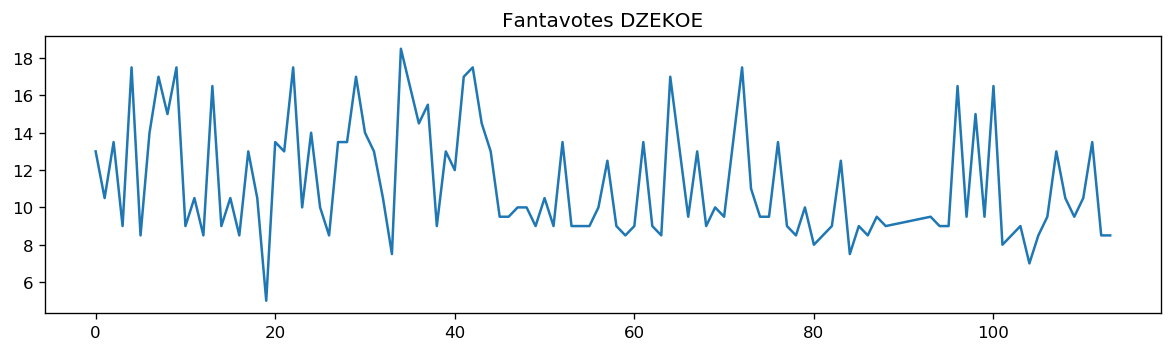
\includegraphics[scale=0.5]{images/dzeko_linear_interpolation_fantavotes.png}
   \centering  
   \caption{\textit{Fantavotes of ''Edin Dzeko'' with \textit{linear interpolation}}}
  \label{fig:linear_interpolation}
\end{figure}

\begin{figure}[H]
  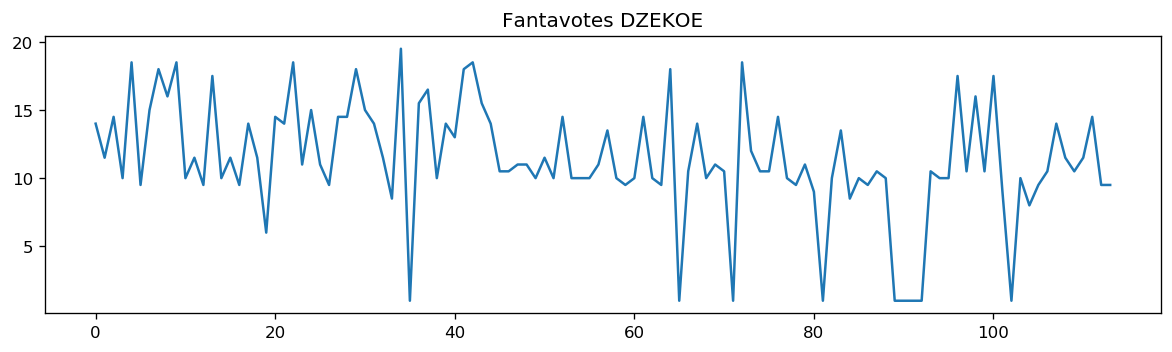
\includegraphics[scale=0.5]{images/dzeko_placeholder_fantavotes.png}
   \centering  
   \caption{\textit{Fantavotes of ''Edin Dzeko'' with \textit{placeholder}}}
  \label{fig:placeholder}
\end{figure}

\section{Translation}

Votes are translated coherently in order to yield them in a positive range.
\\
This is useful e.g. when applying log transform operations. 


\chapter {Analysis on players data}

The previous phases of data cleaning resulted in a dataset of 917 players with 114 votes each.
Analysis are performed on different abstraction levels.
At the beginning, high-level evaluations are made to discover stats on number of played matches (mean, min, max etc.); analysis on number of played matches are reported in figure \ref{fig:countMatch}.
\\
\begin{figure}[H]
  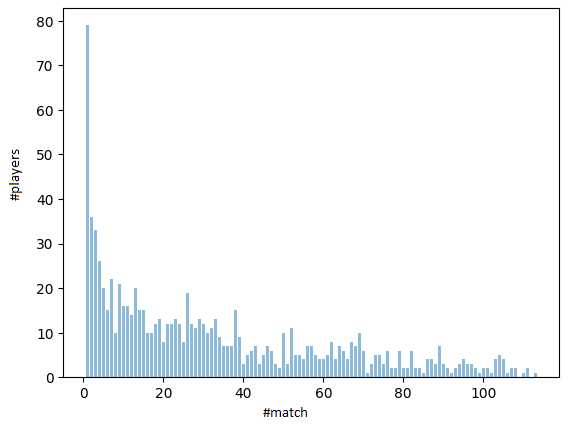
\includegraphics[scale=0.9]{images/img-01.png}
   \caption{\textit{Count number of players that played a certain number of matches.}}
  \label{fig:countMatch}
\end{figure}

Similarly, a fine grained analysis has been made by grouping players per role, as shown in figure \ref{fig:countMatchPerRole}, but no relevant differences have been found.

\begin{figure}[H]
  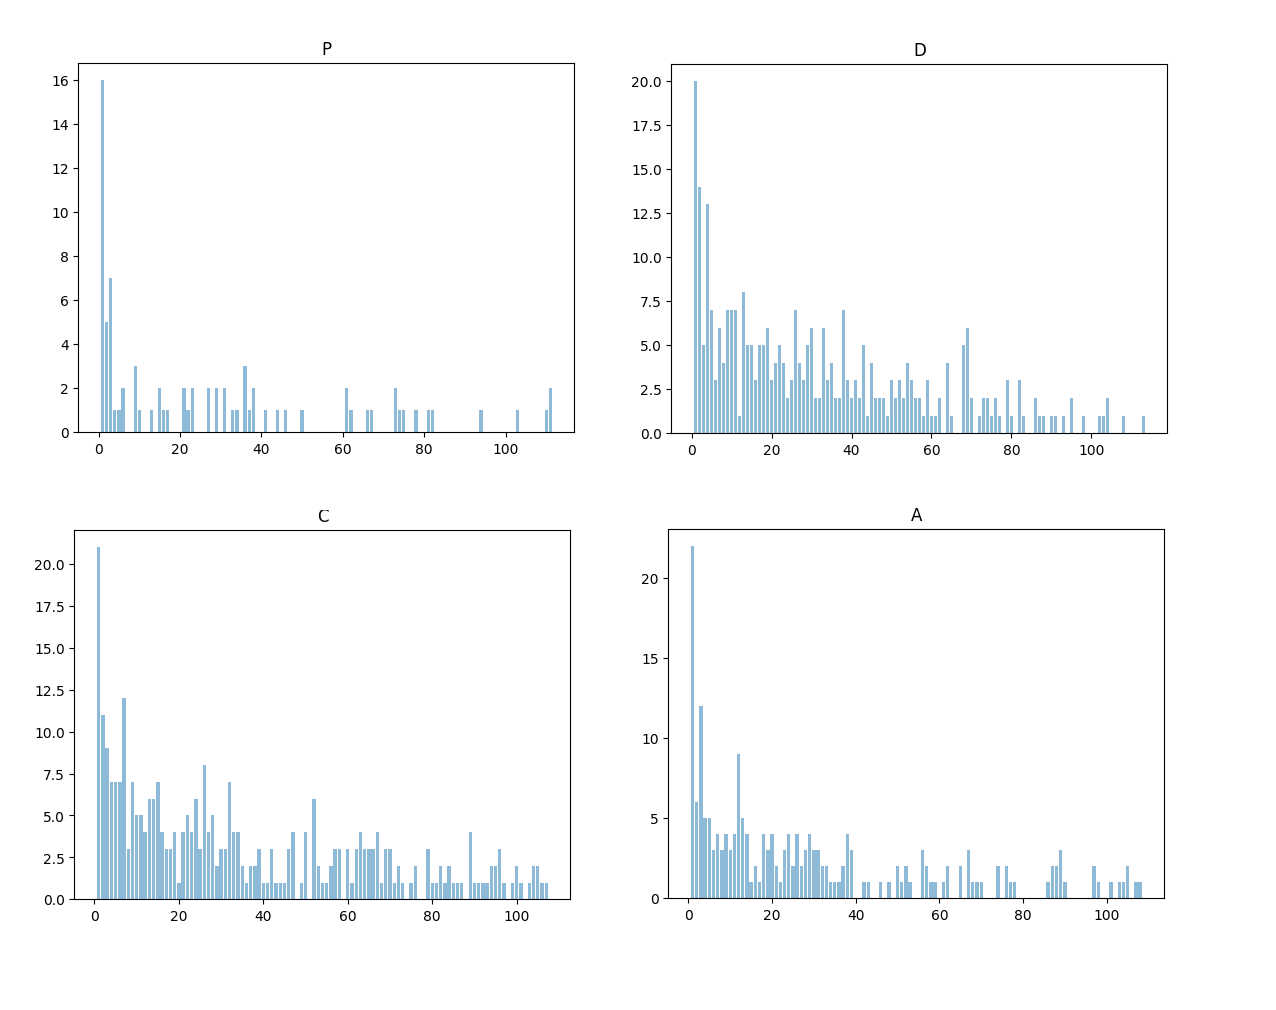
\includegraphics[scale=0.4]{images/img-02.png}
   \caption{\textit{Count number of players of such role that played a certain number of matches.
   Legend: P = Goalkeeper, D = Defender, C = Midfielder, A = Striker}}
  \label{fig:countMatchPerRole}
\end{figure}

\newpage
\section{Data correlation}

The task goal is discovering, if present, seasonality on players' votes.
\\
In order to achieve such a target, Pearson Correlation Index has been used, for single player and for role both.
\\
Empirical tests show that no relevant seasonality can be detected.
\\
Figure \ref{fig:playereg} reports data on an example player.

\begin{figure}[H]
  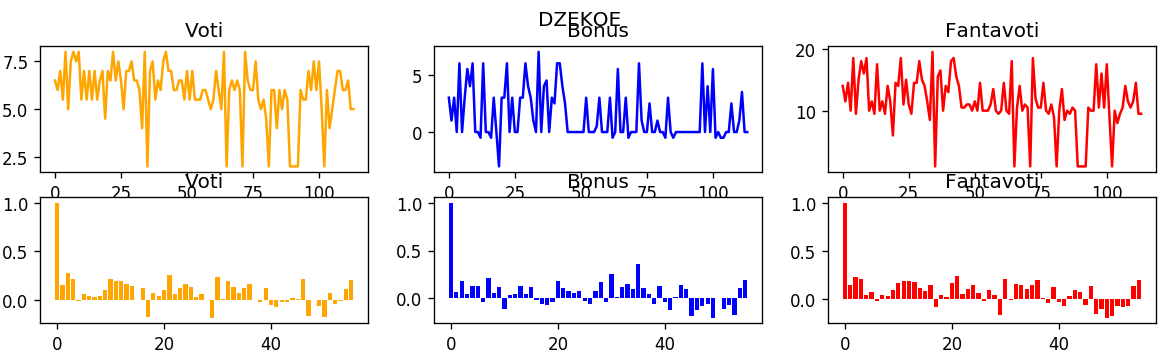
\includegraphics[scale=0.5]{images/img-03.png}
   \caption{\textit{The image shows storic series and respective Pearson correlations for ''Edin Dzeko''.}}
  \label{fig:playereg}
\end{figure}

\section{Normality test}

Normalty test were made on both votes and fantavotes to determine if the two datasets could be modeled by a normal distribution.
qq-plot and histograms of votes showed a correlation with the normal distribution for almost all players  (Figure \ref{fig:hist_votes} and Figure \ref{fig:qqplot_votes})
The same can't be said for the fantavotes dataset (Figure \ref{fig:hist_fantavotes} and Figure \ref{fig:qqplot_fantavotes})

\begin{figure}[H]
  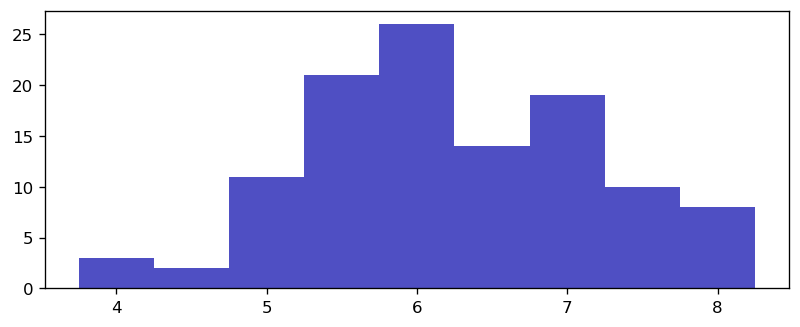
\includegraphics[scale=0.5]{images/dzeko_normality_test_voti_barchart.png}
    \centering  
   \caption{\textit{'Votes' histogram for ''Edin Dzeko''.}}
  \label{fig:hist_votes}
\end{figure}

\begin{figure}[H]
  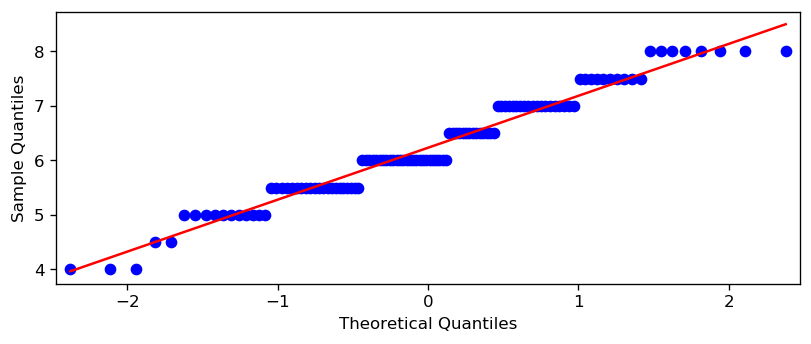
\includegraphics[scale=0.5]{images/dzeko_normality_test_voti_qqplot.png}
   \centering  
   \caption{\textit{'Votes' qqplot for ''Edin Dzeko''.}}
  \label{fig:qqplot_votes}
\end{figure}

\begin{figure}[H]
  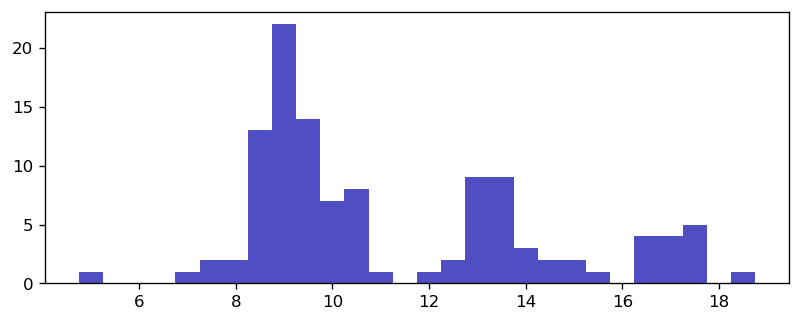
\includegraphics[scale=0.5]{images/dzeko_normality_test_fantavoti_barchart.png}
   \centering  
   \caption{\textit{'Fantavotes' histogram for ''Edin Dzeko''.}}
  \label{fig:hist_fantavotes}
\end{figure}

\begin{figure}[H]
  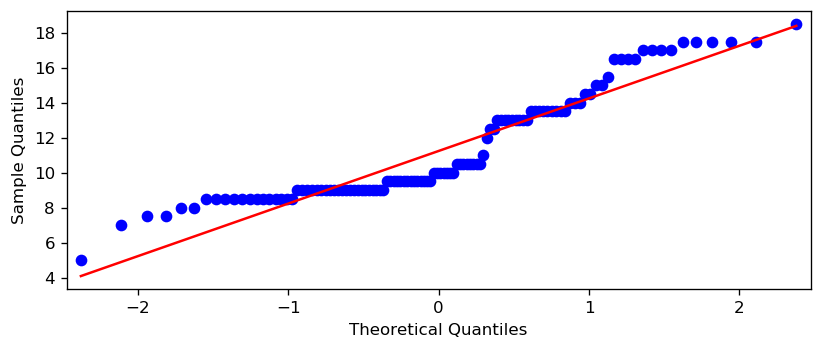
\includegraphics[scale=0.5]{images/dzeko_normality_test_fantavoti_qqplot.png}
   \centering  
   \caption{\textit{'Fantavotes' qqplot for ''Edin Dzeko''.}}
  \label{fig:qqplot_fantavotes}
\end{figure}






  
\chapter {Forecast}

The forecasting has been implemented in two differents ways: SARIMA and MLP.
We have chosen to work on a smaller subset of data to speed up the comparison phase between the models.
The dataset used in forecasting evaluation is composed in fact by the players present in all three seasons and numer of matches played greater then 100.
The result is a 25 players dataset. 
Each player's fantavotes has been divided into train set and test set (70\% - 30\%).
The performances are compared in table \ref{table:RMSE} using \textit{Root Mean Squared Error} (RMSE) as common metric.

\section{SARIMA}

Regarding SARIMA, \textit{auto-arima} function has been used to find the best parameters for the ARIMA model.
An example of application of the sarima model is visible in Figure \ref{fig:sarima}


\begin{figure}[H]
  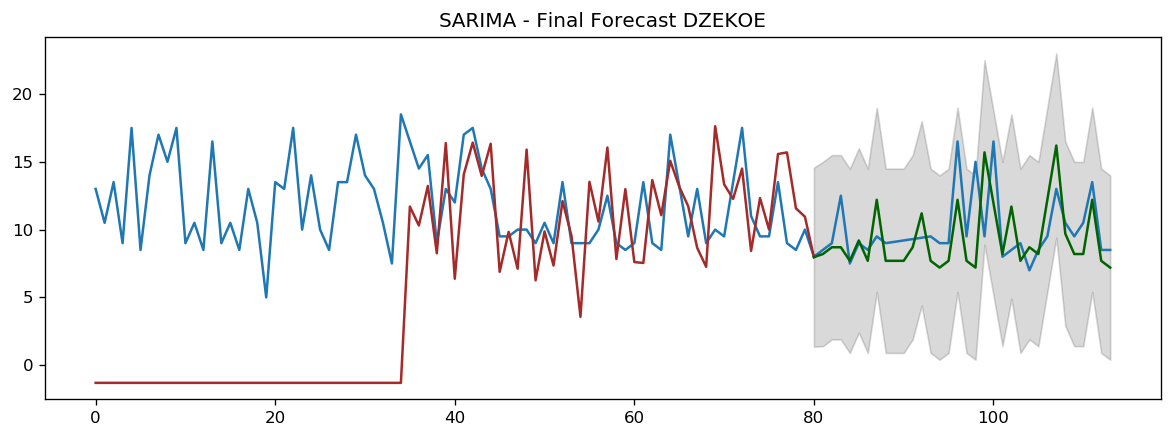
\includegraphics[scale=0.5]{images/dzeko_sarima_fantavoti.png}
   \caption{\textit{SARIMA forecast on ''Edin Dzeko''.}}
  \label{fig:sarima}
\end{figure}

\section{MLP}
The MLP model architecture includes 1 input layer with 12 nodes, 1 hidden layer with 38 nodes and 1 output layers with 1 node. The activation function is \textit{relu}.
The network has been trained with Adam optimizer and 150 epochs.
An example of application of the mlp model is visible in Figure \ref{fig:mlp}
\begin{figure}[H]
  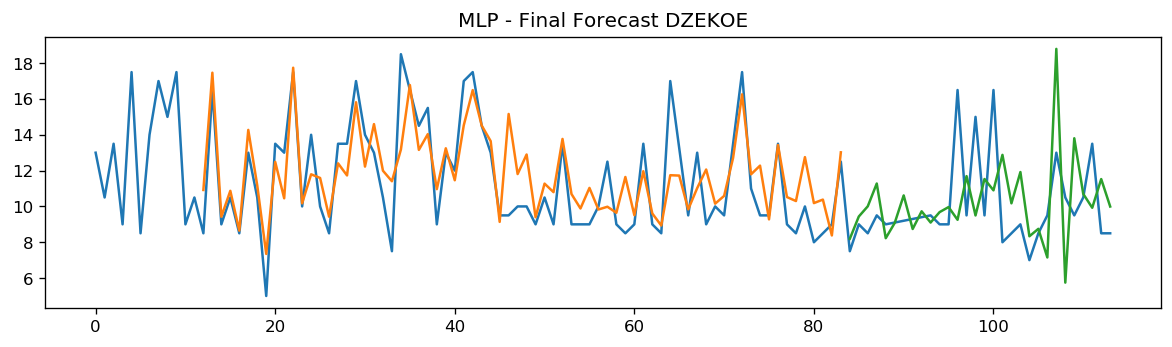
\includegraphics[scale=0.5]{images/dzeko_mlp_fantavoti.png}
   \caption{\textit{MLP forecast on ''Edin Dzeko''.}}
  \label{fig:mlp}
\end{figure}

\section{Models combination}

In order to improve accuracy (\textit{rmse}) on predictions, the two models were ensembled to come up with an hybrid version.
The final model used for forecasting is defined as:
\\
\begin{center}
  $\alpha * MLP + (1 - \alpha) * SARIMA$
\end{center}
where:
\begin{itemize}
    \item \textbf{$\alpha$} is a costant weight between 0 and 1 and is the value that minimizes the RMSE
    \item \textbf{MLP} is the value predicted by MLP model
    \item \textbf{SARIMA}  is the value predicted by SARIMA model 
\end{itemize}


\begin{figure}[H]
  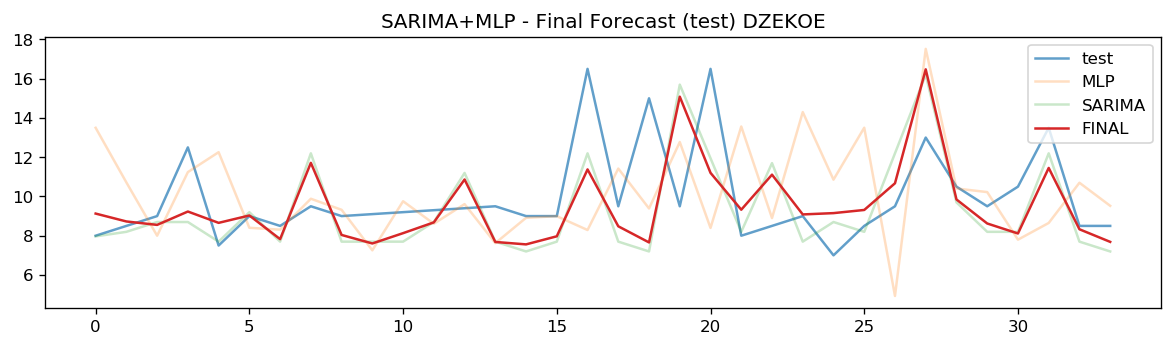
\includegraphics[scale=0.5]{images/dzeko_final_forecast.png}
   \caption{\textit{Final forecast on test set of ''Edin Dzeko''. $\alpha  = 0.21$, \textit{linear interpolation}}}
  \label{fig:mlp}
\end{figure}

\begin{figure}[H]
  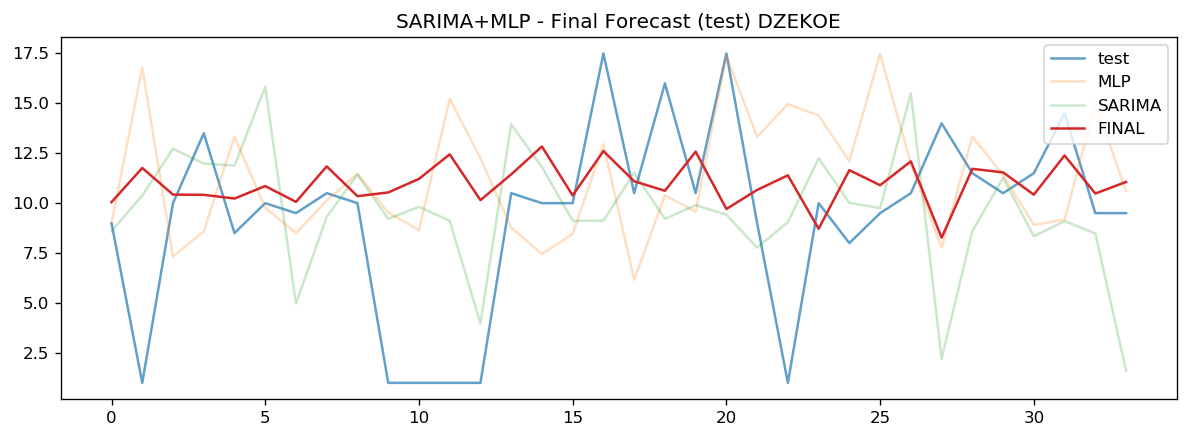
\includegraphics[scale=0.5]{images/dzeko_final_forecast_placeholder.png}
   \caption{\textit{Final forecast on test set of ''Edin Dzeko''. $\alpha  = 0.21$, \textit{placeholder}}}
  \label{fig:mlp}
\end{figure}



\begin{table}
 \begin{tabular}{|c|c|c|c|} 
 \hline
 Filling method & SARIMA+MLP & SARIMA & MLP \\
 \hline \hline
 Linear interpolation & 1.94 & 1.97 & 2.21 \\
 Placeholder & 3.48 & 4.22 & 4.31 \\
 \hline
 \end{tabular}
 \caption{\textit{Comparison between different models and filling methods using RMSE.}}
 \label{table:RMSE}
\end{table}









	
\backmatter	

\end{document}